
%---------------------------------------------------------------------------------------
%	PACKAGES AND OTHER DOCUMENT CONFIGURATIONS
%----------------------------------------------------------------------------------------
\documentclass[a0,portrait]{a0poster}
%%
\usepackage[top=5cm, bottom=0.3cm, left=5cm, right=3cm]{geometry}
\usepackage[compact]{titlesec}
\usepackage{multicol} % This is so we can have multiple columns of text side-by-side
\columnsep=100pt % This is the amount of white space between the columns in the poster
\columnseprule=20pt % This is the thickness of the line between the columns in the poster
%\usepackage[svgnames]{xcolor} % Specify colors by their 'svgnames', for a full list of all colors available see here: http://www.latextemplates.com/svgnames-colors
%\usepackage{times} % Use the times font
\usepackage{palatino} % Uncomment to use the Palatino font
\usepackage{xkeyval}
\usepackage{graphicx} % Required for including images
\setlength{\abovecaptionskip}{5pt plus 5pt minus 3pt}
\graphicspath{{figures/}} % Location of the graphics files
\usepackage{booktabs} % Top and bottom rules for table
\usepackage[font=small,labelfont=bf]{caption} % Required for specifying captions to tables and figures
\usepackage{amsfonts, amsmath, amsthm, amssymb} % For math fonts, symbols and environments
%\usepackage[pdftex]{color}
\usepackage{framed}
\usepackage[utf8]{inputenc}
\usepackage[T1]{fontenc}
\usepackage{csquotes}
\usepackage{booktabs}
\usepackage[portuguese]{babel}
\usepackage{wrapfig} % Allows wrapping text around tables and figures
\usepackage[usenames, dvipsnames]{xcolor}
\definecolor{sematcolor2}{rgb}{0.09, 0.41, 0.56}
\definecolor{sematcolor}{rgb}{0.05, 0.25, 0.50}
\definecolor{sematcolor3}{rgb}{0.24, 0.82, 0.98}
\colorlet{frameborder}{sematcolor2}
\def\columnseprulecolor{\color{sematcolor}}%

\usepackage{mdframed}
\usepackage{xcolor}

\newmdenv[
hidealllines=true,
backgroundcolor=sematcolor3,
topline=true,
bottomline=true,
linewidth=5pt,
linecolor=sematcolor
]{mybox}

\newmdenv[
hidealllines=true,
backgroundcolor=sematcolor,
topline=true,
bottomline=true,
linewidth=5pt,
linecolor=sematcolor
]{mydarkbox}

\usepackage{amsthm, amsmath, wasysym, MnSymbol}

\newtheorem{theorem}{Teorema}
\newtheorem{proposition}[theorem]{Proposição}
\newtheorem{lemma}[theorem]{Lema}
\newtheorem{definition}[theorem]{Definição}
\newtheorem{corollary}[theorem]{Corolário}
\renewcommand{\qedsymbol}{$\blacksquare$}





%----------------------------------------------------------------------------------------
%	POSTER HEADER 
%----------------------------------------------------------------------------------------
% The header is divided into three boxes:
% The widths of these boxes can be easily edited to accommodate your content as you see fit
\begin{document}
%\hspace*{0.2cm}
\begin{minipage}[c]{\linewidth}
\vspace{0.1cm}
\noindent\makebox[\textwidth][c]{
\begin{minipage}[c]{0.10\linewidth}
\vspace{0pt}\raggedright
\hspace{1cm}
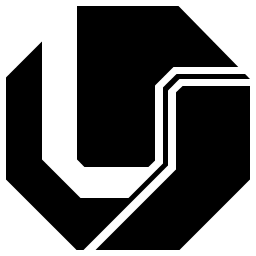
\includegraphics[width=\linewidth]{ufulogo}
\end{minipage}
\hfill
\begin{minipage}[c]{0.70\textwidth}
\centering
\Huge \color{sematcolor} \textbf{Análise numérica da equação da difusão bidimensional transiente pelo método explícito}\\[1cm]
\Large \color{Black} \textbf{\underline{Felipe José Oliveira Ribeiro}, Ítalo Augusto Magalhães de Ávila Ribeiro, Hélio Ribeiro Neto e Aristeu da Silveira Neto}\\[1cm] % Author(s)
\normalsize Faculdade de Engenharia Mecânica, UFU, Uberlândia-MG\\[0.1cm] % University

\small \texttt{Contato:feliperibeiro.ufu@gmail.com}\\
\end{minipage}
%\hfill
\begin{minipage}[c]{0.17\textwidth}
\vspace{0pt}\raggedleft
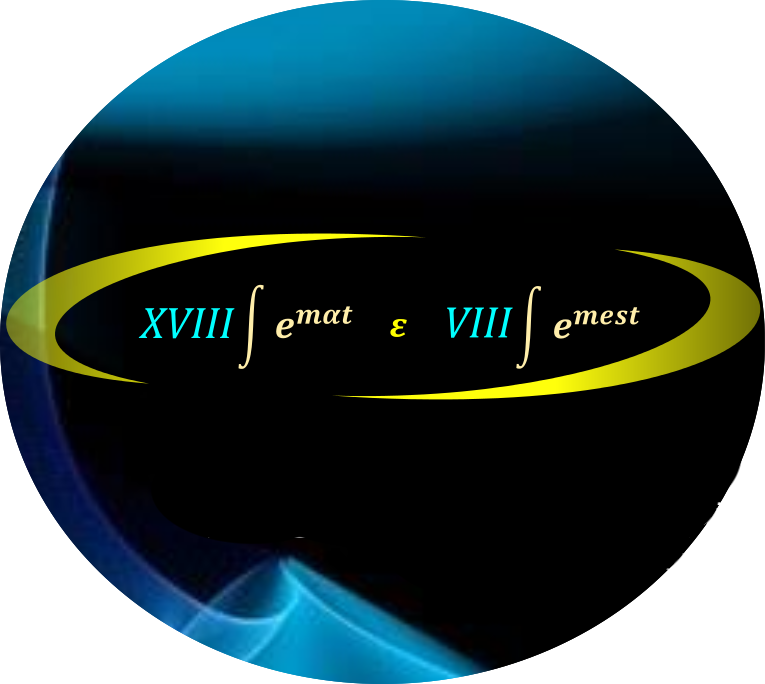
\includegraphics[scale=0.33]{fundologo}
\hspace{1cm}
\end{minipage}}
\\[0.1cm]%
% A bit of extra whitespace between the header and poster content
%----------------------------------------------------------------------------------------
\color{sematcolor}\setlength\FrameRule{25pt}
\begin{framed}
\vspace{0.5cm}
\begin{multicols}{2} % This is how many columns your poster will be broken into, a portrait poster is generally split into 2 columns







%----------------------------------------------------------------------------------------
%	INTRODUCTION
%----------------------------------------------------------------------------------------
\color{Black}
\section*{Introdução}
%Lorem ipsum dolor sit amet, consectetur adipiscing elit, sed do eiusmod tempor incididunt ut labore et dolore magna aliqua. 
%\begin{mybox}
%\begin{lemma}
%Duis aute irure dolor in reprehenderit in voluptate velit esse cillum dolore eu fugiat nulla pariatur. 
%\end{lemma}
%\end{mybox}
%Ut enim ad minim veniam, quis nostrud exercitation ullamco laboris nisi ut aliquip ex ea commodo consequat.
%\begin{mybox}
%\begin{theorem}
%Lorem ipsum dolor sit amet, consectetur adipiscing elit, sed do eiusmod tempor incididunt ut labore. Ut enim ad minim veniam, quis nostrud exercitation ullamco laboris nisi ut aliquip ex ea commodo consequat.
%\end{theorem}
%\end{mybox}
%Excepteur sint occaecat cupidatat non proident, sunt in culpa qui officia deserunt mollit anim id est laborum (Fig.-\ref{IGSMap}) Lorem ipsum dolor sit amet, consectetur adipiscing elit, sed do eiusmod tempor incididunt ut labore et dolore magna aliqua.  Duis aute irure dolor in reprehenderit in voluptate velit esse cillum dolore eu fugiat nulla pariatur. Excepteur sint occaecat cupidatat non proident, sunt in culpa qui officia deserunt mollit anim id est laborum.\\
%%\begin{wrapfigure}{R}{0.25\textwidth}
%\begin{center}
%\hspace*{\fill}
%
\includegraphics[width=0.49\linewidth]{figures/placeholder}
%
\includegraphics[width=0.49\linewidth]{figures/placeholder}
%\captionof{figure}{\color{sematcolor2}(left) Lorem ipsum dolor sit amet, consectetur adipiscing elit, sed do eiusmod tempor incididunt ut labore et dolore magna aliqua. Ut enim ad minim veniam, quis nostrud exercitation ullamco laboris nisi \textendash re Excepteur sint occaecat cupidatat non proident, sunt in culpa qui officia deserunt mollit anim id est laborum.}
%\label{IGSMap}
%\end{center}
%In this contributionLorem ipsum dolor sit amet, consectetur liquip ex ea commodo consequat. Duis aute irure dolor in reprehenderit in voluptate velit esse cillum dolore eu fugiat nulla pariatur. Excepteur sint occaecat cupidatat non proident, sunt in culpa qui officia deserunt mollit anim id est laborum.

Muitos fenômenos físicos podem ser modelados, isto é, representados matematicamente, por meio de Equações Diferenciais Parciais (EDPs). A sua solução por métodos analíticos, no entanto, é limitada a casos lineares e simples, que não representam de maneira satisfatória a maioria dos fenômenos físicos. O método numérico é empregado como alternativa para a solução de problemas de maior complexidade. Um exemplo é a solução da equação da energia térmica em regime transiente. Na literatura da área, existem vários métodos de solução numérica de equações diferenciais. São exemplos o Método dos Elementos Finitos, Método dos Volumes Finitos e Método de Diferenças Finitas. Em tais métodos, o domínio é discretizado e as relações diferenciais são aproximadas por um sistema  algébrico de equações. Tal aproximação implica em um erro em relação à solução exata, o qual pode ser quantificado sob determinadas condições. No presente trabalho, procura-se apresentar um estudo de caso para a análise de erro envolvendo a resolução da EDP que modela a equação da energia térmica em um domínio bidimensional. 


%----------------------------------------------------------------------------------------
%	METHODS
%---------------------------------------------------------------------------------------- 
\color{Black}
\section*{Método numérico}
%\begin{wrapfigure}{R}{0.25\textwidth} % R é o parametro que coloca a figura a direita do texto, para esquerda troque por L. 0.25\textwidth define a largura como 25 por cento do largura do texto do poster.
%\centering
%
\includegraphics[scale=0.5]{figures/placeholder}
%\captionof{figure}{\color{sematcolor2}Loreteur sint occaecat cupidatat non proident, sunt in culpa qui officia deserunt mollit anim id est laborum.}
%\label{STECchart}
%\end{wrapfigure}
%Key information about the sources of data and methods employed in the study are highlighted below.\\
%\hspace{0.1cm}$\circ$ Sdfshd d: 25\textendash31 January, 2015;\\
%\hspace{0.1cm}$\circ$ Redfshdghgons (Fig.\ref{IGSMap}): Lorem ipsum dolor sit amet, consectetur adipiscing elit, sed;\\
%\hspace{0.1cm}$\circ$ Geomagnetic activity: Kp $<$ 4 throughout the study period;\\
%\hspace{0.1cm}$\circ$ Analysis: Two types of accuracy and;\\
%\hspace{0.1cm}$\circ$ GIR: Lorem ipsum dolor sit amet, consectetur adipiscing elit, sed do eiusmod tempor;\\
%\hspace{0.1cm}$\circ$ AGD: Lsunt in culpa qui officia deserunt mollit anim id est laborum.\\
%
%\begin{mybox}
%\begin{proposition}
%Num triângulo retângulo, o quadrado da medida da hipotenusa é igual à soma dos quadrados das medidas dos catetos.
%\end{proposition}
%\end{mybox}
Na equação da difusão, para o caso bidimensional (indicada abaixo), aparecem duas parcelas diferenciais. 
\begin{equation} \label{difusao_pura}
\frac{\partial \phi}{\partial t} = \alpha \,\left( \frac{\partial^{2} \phi}{\partial x^{2}} + \frac{\partial^{2} \phi}{\partial y^{2}} \right) 
\end{equation}
Na qual $\phi$ é a variável a ser transportada, função do tempo $t$ e das variáveis espaciais $x$ e $y$, $\alpha$ é uma constante, a qual pode representar o coeficiente de difusividade de uma dada informação.
Utilizando a expansão em série de Taylor para a discretização do termo diferencial de primeira ordem, faz-se uso da equação acima para a expansão da função no domínio do tempo:

\begin{equation} \label{Time_discretization}
\frac{\phi \left(t+\Delta t, x, y \right)-\phi \left(t, x, y\right)}{\Delta t}= \frac{\partial \phi \left(t, x, y\right)}{\partial t} + \sum\limits_{n=2}^{\infty} \frac{\Delta t^{n-1}}{n!} \frac{\partial^{n} \phi\left(t, x, y\right)}{\partial t^{n}}.
\end{equation}
Truncando a equação \ref{Time_discretization} no termo de primeira ordem ($\mathcal{O}(\Delta t)$), obtém-se o método de Euler explícito.
Analogamente, a discretização para os termos de segunda ordem é obtida, fazendo uso de um incremento e um decremento no espaço, enquanto o tempo é fixado, obtendo-se a discretização para a derivada segunda em uma das direções. 

\begin{equation} \label{Spacial_discretization3}
\frac{\phi \left(t, x+\Delta x, y\right)-2 \phi \left(t, x, y\right) + \phi \left(t, x-\Delta x\right)}{\Delta x^2} = \\
\frac{\partial^{2} \phi \left(t, x, y\right)}{\partial x^{2}}+ \\
2 \sum\limits_{n=2}^{\infty} \frac{ \Delta x^{\left(2\left(n-1\right)\right)}}{\left(2n\right)!} \frac{\partial^{\left(2n\right)} \phi \left(t, x, y\right)}{\partial x^{\left(2n\right)}}.
\end{equation}
A mesma metodologia empregada em $x$ é estendida à dimensão $y$.
Substituindo as relações truncadas na equação \ref{difusao_pura} tem-se a equação \ref{difusao_discretizada} .
\begin{equation} \label{difusao_discretizada}
\begin{split}
\frac{\phi \left(t+\Delta t, x, y\right)-\phi \left(t, x, y\right)}{\Delta t} \ - \ &\alpha \left( \frac{\phi \left(t, x+ \Delta x, y \right)-2 \phi \left(t, x, y \right) + \phi \left(t, x- \Delta x, y \right)}{\Delta x^2} \right) -\\
&\alpha \left( \frac{\phi \left(t, x, y+ \Delta y \right)-2 \phi \left(t, x, y \right) + \phi \left(t, x, y- \Delta y \right)}{\Delta y^2} \right) \approx 0 .% + g\left(x,t\right)
\end{split}
\end{equation}


A solução numérica requer a discretização dos domínios espacial e temporal. Ou seja, deve-se traduzir um
conjunto contínuo e infinito de informações em um conjunto discreto e finito, no qual é empregada a metodologia numérica. Os domínios espacial e temporal são discretizados uniformemente. Assim, para $(t,x,y) \in [a,b] \times [c,d] \times [e,f]$, consideramos: $t^{N} = N \Delta t, (\ \ N=0,1,2,...,M,)$ , $x_{I} = I \Delta x,(\ \ I=0,1,2,...,L,)$, $y_{J} = J \Delta y, (\ \ J=0,1,2,...,O, )$ , onde $M$, $L$ e $O$ são o número de divisões nos intervalos $[a,b]$, $[c,d]$ e $[e,f]$, respectivamente.
É conveniente definir a solução numérica para os pontos discretos $\Phi_{I,J}^{N}$, que não é idêntica à solução analítica de $\phi (x,y,t)$. Assim, é possível reescrever a equação \ref{difusao_discretizada} como indicado à
seguir.

\begin{equation} \label{numerical_sol}
\begin{split}
\frac{\Phi_{I,J}^{N+1}-\Phi_{I,J}^{N} }{\Delta t} - \alpha \left( \frac{\Phi_{I+1,J}^{N} -2 \Phi_{I,J}^{N} + \Phi_{I-1,J}^{N}}{\Delta x^2} \right) -	\alpha \left( \frac{\Phi_{I,J+1}^{N}-2 \Phi_{I,J}^{N} + \Phi_{I,J-1}^{N}}{\Delta y^2} \right) = 0. % + g\left(x,t\right)
\end{split}
\end{equation}

 Define-se uma função $\psi(t,x,y)$ que é contínua e coincidente com a solução no ponto discreto ($N,I,J$) e é diferente da solução exata $\phi(t,x,y)$. Em outras palavras, $\phi(t,x,y)$ é a solução exata, $\Phi_{I,J}^{N}$ é a solução aproximada, obtida do sistema discreto, e $\psi(t,x,y)$ é a solução contínua que está de acordo com a obtida por $\Phi$ no ponto (respectivos $N$, $I$ e $J$) e que é diferente de $\phi(t,x,y)$. Substituindo $\Phi_{I,J}^{N}$ na equação \ref{numerical_sol} por $\psi(t,x,y)$ e expandindo os termos em série de Taylor ao redor do ponto $(t,x,y)$, obtém-se a equação apresentada à seguir.	

\begin{equation} \label{difusao_continuum}
\begin{split}
\frac{\partial \psi}{\partial t} - \alpha \left( \frac{\partial^{2} \psi}{\partial x^{2}} + \frac{\partial^{2} \psi}{\partial y^{2}} \right) = 2 \alpha \sum\limits_{n=2}^{\infty} \frac{ \Delta x^{\left(2\left(n-1\right)\right)}}{\left(2n\right)!} \frac{\partial^{\left(2n\right)} \psi \left(t, x, y\right)}{\partial x^{\left(2n\right)}} + 2 \alpha \sum\limits_{n=2}^{\infty} \frac{ \Delta y^{\left(2\left(n-1\right)\right)}}{\left(2n\right)!} \frac{\partial^{\left(2n\right)} \psi \left(t, x, y\right)}{\partial y^{\left(2n\right)}} \\ - \sum\limits_{n=2}^{\infty} \frac{\Delta t^{n-1}}{n!} \frac{\partial^{n} \psi\left(t, x, y\right)}{\partial t^{n}}. % + g\left(x,t\right)
\end{split}
\end{equation}
O lado direito da equação \ref{difusao_continuum} expressa o erro numérico da discretização segundo a metodologia explícita. Tal relação é apresentada em função de termos espaciais e temporais. Visando facilitar a análise, procura-se reescrever a relação em função apenas de termos do domínio espacial. Assim, deve-se empregar sistematicamente a equação \ref{difusao_continuum} na simplificação dos termos desejados. Truncando termos de ordem superior a 4 tem-se:

\begin{equation} \label{difusao_continuum2}
\frac{\partial \psi}{\partial t} - \alpha \left(\frac{\partial^{2} \psi}{\partial x^{2}} + \frac{\partial^{2} \psi}{\partial y^{2}} \right) + \frac{\Delta t}{2} \frac{\partial^{2} \psi}{\partial t^{2}} + \frac{\Delta t^{2}}{6} \frac{\partial^{3} \psi}{\partial t^{3}} - \alpha \frac{\Delta x^{2}}{12} \frac{\partial^{4} \psi}{\partial x^{4}} - \alpha \frac{\Delta x^{4}}{60} \frac{\partial^{6} \psi}{\partial x^{6}} - \alpha \frac{\Delta y^{2}}{12} \frac{\partial^{4} \psi}{\partial y^{4}} - \alpha \frac{\Delta y^{4}}{60} \frac{\partial^{6} \psi}{\partial y^{6}} +  ... = 0.
\end{equation}

Uma série de derivações algébricas são levadas. A resultante é indicada à seguir.

\begin{equation} \label{termo_temporal_tres}
\begin{split}
&\frac{\partial \psi}{\partial t} - \alpha \left(\frac{\partial^{2} \psi}{\partial x^{2}} + \frac{\partial^{2} \psi}{\partial y^{2}} \right) +\frac{\Delta t^{3}}{12} \frac{\partial^{4}\psi}{\partial t^{4}} + \frac{\Delta t^{4}}{2(6!)} \frac{\partial^{5}\psi}{\partial t^{5}}- 2 \frac{\alpha \Delta x^{2}}{4!} \frac{\partial^{4} \psi}{\partial x^{4}} - 2 \frac{\alpha \Delta y^{2}}{4!} \frac{\partial^{4} \psi}{\partial y^{4}} - 2 \frac{\alpha \Delta x^{4}}{6!} \frac{\partial^{6} \psi}{\partial x^{6}} - \\
&2 \frac{\alpha \Delta y^{4}}{6!} \frac{\partial^{6} \psi}{\partial y^{6}} - \alpha \frac{\Delta t}{2} \frac{\partial^{3} \psi}{\partial x^{2} \partial t} + \alpha \frac{\Delta t}{2} \frac{\partial^{3} \psi}{\partial y^{2} \partial t} - \frac{\Delta x^{2} \Delta t}{48} \frac{\partial^{4} \psi}{\partial x^{4} \partial t} - \frac{\Delta y^{2} \Delta t}{48} \frac{\partial^{4} \psi}{\partial y^{4} \partial t}  +... = 0.
\end{split}
\end{equation}	
Para cancelar as derivadas parciais nas duas dimensões, faz-se uso do teorema de Clairaut-Schwarz (inversão da ordem de derivação). Essa metodologia deve ser empregada até que todas as derivadas parciais no tempo sejam suprimidas da equação truncada. Por fim, chega-se a equação modificada, que é apresentada abaixo.

\begin{equation} \label{termo_temporal_quatro}
\begin{split}
\frac{\partial \psi}{\partial t} - \alpha \left(\frac{\partial^{2} \psi}{\partial x^{2}} + \frac{\partial^{2} \psi}{\partial y^{2}} \right) = 2\alpha \left(\frac{\Delta x^{2}}{4!} +\frac{\alpha \Delta t}{4}\right) \frac{\partial^{4}\psi}{\partial x^{4}} +2\alpha \left(\frac{\Delta y^{2}}{4!} +\frac{\alpha \Delta t}{4}\right) \frac{\partial^{4}\psi}{\partial y^{4}} \\  +2 \alpha \left(\frac{\Delta x^{4}}{6!} - \frac{\alpha \Delta x^{2}\Delta t}{2(4!)} + \frac{\alpha \Delta x^{4}\Delta t}{48}\right) \frac{\partial^{6}\psi}{\partial x^{6}} + 2\alpha \left(\frac{\Delta y^{4}}{6!}- \frac{\alpha \Delta y^{2}\Delta t}{2(4!)} + \frac{\alpha \Delta y^{4}\Delta t}{48}\right) \frac{\partial^{6}\psi}{\partial y^{6}} \\ + 2 \alpha \left(\frac{\Delta x^{6}}{8!} - \frac{\alpha \Delta x^{4}\Delta t}{2(6!)} + \frac{\alpha \Delta x^{6}\Delta t}{48(4!)} \right) \frac{\partial^{8}\psi}{\partial x^{8}} + 2 \alpha \left(\frac{\Delta y^{6}}{8!} - \frac{\alpha \Delta y^{4}\Delta t}{2(6!)} + \frac{\alpha \Delta y^{6}\Delta t}{48(4!)} \right) \frac{\partial^{8}\psi}{\partial y^{8}} + ...
\end{split}
\end{equation}	

Ainda, é possível substituir o passo temporal pelo passo espacial. Define-se uma constante $CFL$, que relaciona o passo temporal aos passos espaciais.
\begin{equation} \label{CFL_one}
\Delta t = \frac{CFL}{\alpha} min[\Delta x^{2}, \Delta y^{2} ] \ \ \ \ \ 
\end{equation}
Substituindo tal condição na equação \ref{termo_temporal_quatro}, e reescrevendo a equação acima de forma conveniente, truncando os termos de ordem superior à quatro, chega-se a equação modificada:


\begin{equation} \label{equacao_modificadaCFL2}
\begin{split}
\frac{\partial \psi}{\partial t} - \alpha \left(\frac{\partial^{2} \psi}{\partial x^{2}} + \frac{\partial^{2} \psi}{\partial y^{2}} \right) = \frac{\alpha \Delta x^{2}}{12} \frac{\partial^{4} \psi}{\partial x^{4}}+ \frac{2 \alpha \Delta x^{4}}{6!} \frac{\partial^{6} \psi}{\partial x^{6}} + \frac{2 \alpha \Delta y^{4}}{6!} \frac{\partial^{6} \psi}{\partial y^{6}} + \frac{\alpha \Delta y^{2}}{12} \frac{\partial^{4} \psi}{\partial y^{4}} \\ + \alpha \ CFL \left[min(\Delta x^{2}, \Delta y^{2})\right] \left(\frac{1}{2} \frac{\partial^{4} \psi}{\partial x^{4}} + \frac{1}{2} \frac{\partial^{4} \psi}{\partial y^{4}} + \frac{1}{4}\frac{\partial^{4} \psi}{\partial x^{2} \partial y^{2}} + \frac{1}{4} \frac{\partial^{4} \psi}{\partial y^{2} \partial x^{2}} \right) \\+ \alpha CFL \left[min(\Delta x^{2}, \Delta y^{2})\right]  \left(\frac{\Delta x^{2}}{4!} \frac{\partial^{6} \psi}{\partial x^{6}} + \frac{\Delta y^{2}}{4!} \frac{\partial^{6} \psi}{\partial y^{6}} + \frac{\Delta x^{2}}{2(4!)} \frac{\partial^{6} \psi}{\partial x^{4} \partial y^{2}} + \frac{\Delta y^{2}}{2(4!)} \frac{\partial^{6} \psi}{\partial x^{4} \partial y^{2}}\right).
\end{split}
\end{equation}

Analisando a equação \ref{equacao_modificadaCFL2}, que apresenta os termos de menores (e mais significativas) ordens do erro numérico, pode-se inferir que o erro é proporcional à condição de $CFL$. Ou seja, o erro é ampliado em função do aumento de tal parâmetro.
%----------------------------------------------------------------------------------------
%	RESULTS
%---------------------------------------------------------------------------------------- 
\color{Black}
\section*{Estudo de caso}
%Fig.-\ref{BIvar} compares tLorem ipsum dolor sit amet, consectetur adipiscing elit, sed do eiusmod tempor incididunt ut labore et dolore magna aliqua. Ut enim ad minim veniam, quis nostrud exercitation ullamco laboris nisi ut aliquip ex ea commodo consequat. Duis aute irure dolor in reprehenderit in voluptate velit esse cillum dolore eu fugiat nulla pariatur. Excepteur sint occaecat cupidatat non proident, sunt in culpa qui officia deserunt mollit anim id est laborum.
%Fig.-\ref{ALICerros} illustrates Lorem ipsum dolor sit amet, consectetur adipiscing elit, sed do eiusmod tempor incididunt ut labore et dolore magna aliqua. Ut enim ad minim veniam, quis nostrud exercitation ullamco laboris nisi ut aliquip ex ea commodo consequat. Duis aute irure dolor in reprehenderit in voluptate velit esse cillum dolore eu fugiat nulla pariatur. Excepteur sint occaecat cupidatat non proident, sunt in culpa qui officia deserunt mollit anim id est laborum.\\
%Lorem ipsum dolor sit amet, consectetur adipiscing elit, sed do eiusmod tempor incididunt ut labore et dolore magna aliqua. Ut enim ad minim veniam, quis nostrud exercitation ullamco laboris nisi ut aliquip ex ea commodo consequat. Duis aute irure dolor in reprehenderit in voluptate velit esse cillum dolore eu fugiat nulla pariatur. Excepteur sint occaecat cupidatat non proident, sunt in culpa qui officia deserunt mollit anim id est laborum
%\begin{center}
%
\includegraphics[width=0.6\linewidth]{figures/placeholder}
%\captionof{figure}{\color{sematcolor2}VLorem ipsum dolor sit amet, ulpa qui officia deserunt mollit anim id est laborumime.}
%\label{GIMupdown}
%\end{center}
%%----------------------------------------------------------------------------------------
%%	CONCLUSIONS
%%----------------------------------------------------------------------------------------
%\color{Black}
Para a solução da equação \ref{numerical_sol} é necessário definir o domínio, condições inicial e de contorno e tempo final de simulação. O domínio espacial escolhido foi de $x=[0,2\pi]$ e $y=[0,2\pi]$ e o tempo final de simulação foi de $10$ segundos.
Para esse estudo de caso, a condição inicial imposta foi:
\begin{equation} \label{condicao_inicial}
\Phi(0,x,y)=U_0 \sin\left(\theta x\right) \sin\left(\theta y\right), %e^{-\alpha \theta^2 t},
\end{equation}
na qual $U_0$ é a amplitude da função e $\theta$ é o número de onda. As condições de contorno foram:
\begin{equation} \label{condicoes_contorno}
\Phi(t,0,y)=0, \ \ \ \Phi(t,2\pi,y)=0,  \ \ \ \Phi(t,x,0)=0, \ \ \ \Phi(t,x,2\pi)=0.
\end{equation}
Para determinar o erro e a convergência do método, comparou-se a solução numérica com a solução analítica:
\begin{equation} \label{solucao_analitica}
\phi(t,x)=U_0 \sin\left(\theta x\right) \sin\left(\theta y\right) e^{-2 \alpha \theta^2 t}.
\end{equation}
Os valores das variáveis $U_0$, $\theta$ e $\alpha$ devem ser escolhidos em função do problema que se deseja resolver. No presente trabalho, o valor escolhido para as três variáveis foi $1,0$. A determinação do erro numérico foi feita, inicialmente, variando o número de divisões espaciais para a condição $CFL = 0,1$. O domínio foi dividido uniformemente nas duas direções ($\Delta x = \Delta y$, com $\Delta x = 2\pi/L = 2\pi/O$). Observa-se na tabela 1 que o erro é reduzido de quatro vezes para o dobro de divisões espaciais em cada direção, comportamento característico de um sistema de segunda ordem, como esperado da análise da equação \ref{equacao_modificadaCFL2}.

\begin{center}
	\captionof{table}{\color{sematcolor2} Dados numéricos de simulação.}
	\begin{tabular}{c|cc|cc|cc}
		\toprule
		Divisões por direção   &  $L_\infty$       	& Razão     & $L_{1}$ 				& Razão 	  $L_{2}$       	& Razão    \\  \toprule
		$25$ 				  & $3,08 \, . 10^{-3}$      & $---$    & $1,48 \, . 10^{-3}$       & $---$         & $1,14 \, . 10^{-3}$      & $---$    \\ 
		$50$ 				  & $7,38 \, . 10^{-4}$      & $4,17$   & $3,62 \, . 10^{-4}$       & $4,09$   	    & $2,87 \, . 10^{-4}$      & $3,97$   \\ 
		$100$ 				  & $1,81 \, . 10^{-4}$      & $4,07$   & $8,96 \, . 10^{-5}$       & $4,04$    	& $7,19 \, . 10^{-5}$      & $3,99$   \\ 
		$200$ 				  & $4,48 \, . 10^{-5}$      & $4,04$   & $2,23 \, . 10^{-5}$       & $4,02$        & $1,80 \, . 10^{-5}$      & $3,99$   \\
		\bottomrule
	\end{tabular}
\end{center}


%\begin{table}[h!]
%	\caption{Erro do método numérico para CFL = 0,1.}
%	\label{tabela1}
%	\centering
%	\begin{tabular}{c | c c c | c c c | c c c}
%		\hline
%		Divisões por direção   &  $L_\infty$       	& Razão   	 & Ordem   & $L_{1}$ 				& Razão 	  & Ordem &  $L_{2}$       	& Razão   	 & Ordem \\ \hline
%		
%		
%		
%		$25$ 				   & $3,08 \, . 10^{-3}$      & $---$   &       $---$   & $1,48 \, . 10^{-3}$       & $---$    	&  $---$     & $1,14 \, . 10^{-3}$      & $---$   & $---$ \\ 
%		
%		
%		$50$ 				  & $7,38 \, . 10^{-4}$      & $4,17$   &       $2,09$  & $3,62 \, . 10^{-4}$       & $4,09$   					&		$2,04$     & $2,87 \, . 10^{-4}$      & $3,97$   & $1,99$\\ 
%		
%		
%		$100$ 				  & $1,81 \, . 10^{-4}$      & $4,07$   &       $2,04$  & $8,96 \, . 10^{-5}$       & $4,04$    		&		$2,02$     & $7,19 \, . 10^{-5}$      & $3,99$   & $2,00$\\ 
%		
%		
%		$200$ 				   & $4,48 \, . 10^{-5}$      & $4,04$   &       $2,02$  & $2,23 \, . 10^{-5}$       & $4,02$    				&		$2, 01$     & $1,80 \, . 10^{-5}$      & $3,99$   & $2,00$\\
%		\hline
%	\end{tabular}
%	
%\end{table}

Segue ainda a avaliação do erro variando-se o $CFL$. O número de divisões para cada direção no domínio espacial foi mantido constante em $50$ para o intervalo $CFL \in [2,5 \ .10^{-3} , 2,5 \ .10^{-1}]$. O resultado obtido é ilustrado à seguir.
\begin{center}
	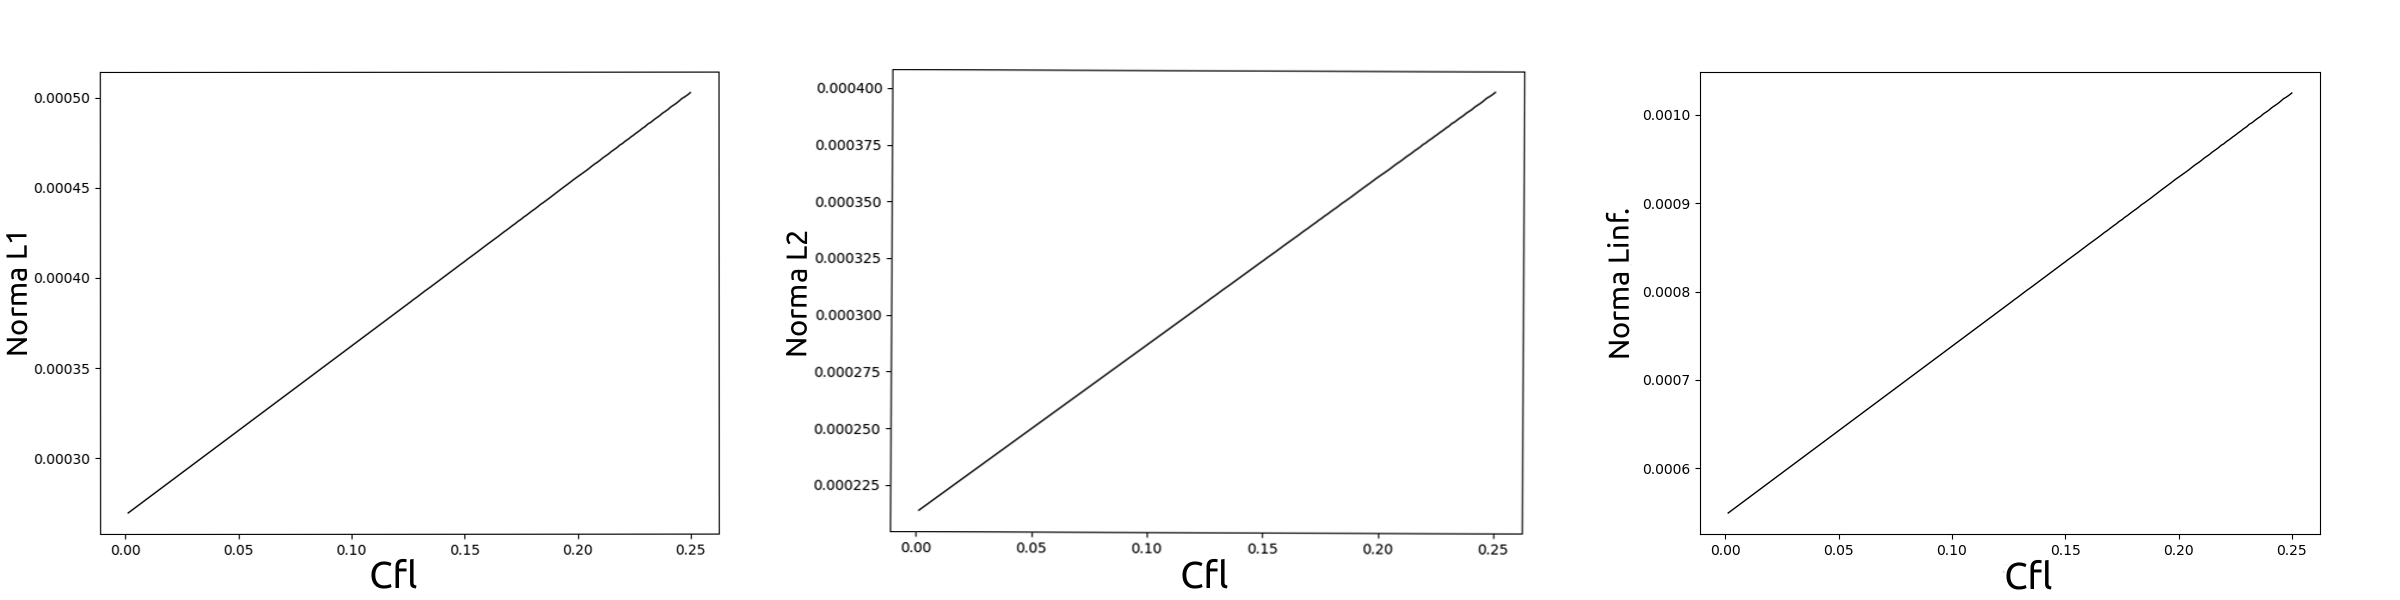
\includegraphics[width=1\linewidth]{NormaL1.png}
	\captionof{figure}{\color{sematcolor2} Erro numérico das simulações em função do $CFL$.}
	\label{fig:erro}
\end{center}
Observa-se na figura 1 que o erro numérico é proporcional ao $CFL$, como esperado pela análise da equação 11.
\section*{Conclusão}

Propôs-se a avaliação de erro para a solução numérica da equação diferencial parcial parabólica que modela o fenômeno da difusão bidimensional em regime transiente. Utilizou-se o método de Euler explícito para a derivada parcial temporal e diferenças centradas para a espacial. Foram feitas a análise numérica do método de discretização e simulações computacionais para avaliar o erro numérico. A solução numérica foi comparada com a solução analítica. Por fim, conclui-se que a parcela de maior representatividade no erro retornado é a do termo de segunda ordem. Ainda, o erro é ampliado em função do aumento da  entre os passos espacial e temporal (definição de $CFL$).

%----------------------------------------------------------------------------------------
%	ACKNOWLEDGEMENTS
%----------------------------------------------------------------------------------------
\section*{Agradecimentos}
Os autores gostariam de agradecer à Petrobras, CAPES, FAPEMIG, CNPq, MFLab e à FEMEC/UFU pelo suporte no desenvolvimento do presente trabalho. 
\end{multicols}
%\textcolor{NavyBlue}{\rule{\linewidth}{15pt}}
\vspace{0.5cm}
\end{framed}
\end{minipage}
%\hspace*{0.1cm}
\end{document}
%----------------------------------------------------------------------------------------
%%%%%%%%%%%%%%%%%%%%%%%%%%%%%%%%%%%%%%%%%%%%%%%%%%